\section*{Autoencoders}
Autoencoders are a subset of neural networks. Whereas a general neural network
 in principle can take any shape, autoencoders are more restrictive.
This restrictiveness can in its most general sence we condensed 
into the following points:
\begin{itemize}
    \item Same number of output categories as input categories  
    \item A latent space with smaller dimensionality than the input/output layer  
\end{itemize}
What we end up with two funnel shaped parts linked together. The two funnels are 
called the encoder (left funnel) and decoder (right funnel) respectively. This architecture is not 
accidental, but rather designed with a very specific solution of ploblems in mind, reconstruction. 
A good example to illustrate this is image denoising, illustrated in figure \ref{fig:ae_denoise}. 
Suppose you have a noised image, and want to denoise it. By feeding the encoder a noised image, 
and comparing the decoder output to the actual image, the autoencoder can tune itself to denoise images. 

\begin{figure}
    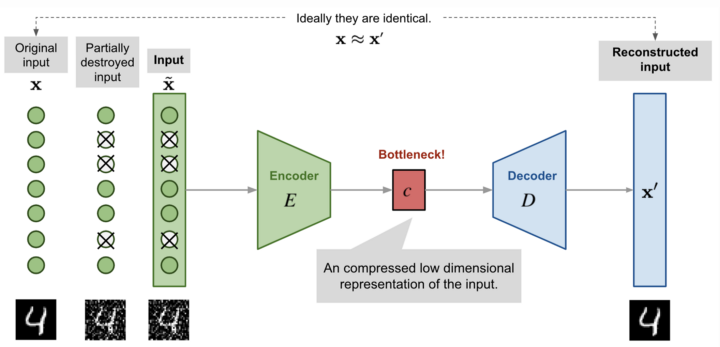
\includegraphics[width=\linewidth]{Figures/Machinelearning/autoencoder_imagedenoising.png}
    \caption{Figure depicting a model for an image denoising autoencoder. Here the input $\bf{x}$ is the original image, $\bf{\tilde{x}}$ is a noised version of $\bf{x}$, $E$ is the encoder, $D$ is the decoder, and $c$ is the latent space. Found 27.09.22 \href{https://miro.medium.com/max/720/0*ECdHu2yeal38Jl3P.png}{here}. }
    \label{fig:ae_denoise}
\end{figure}

Mathematically this is is represented as follows. Using the annotations of each component in figure \ref{fig:ae_denoise}
we have that the decoded information is defined as follows 
\begin{equation*}
    \bf{c} = E_{\phi}(\bf{x}),
\end{equation*}    
and the reconstruction given as 

\begin{equation*}
    \bf{x'} = D_{\theta}(E_{\phi}(\bf{x})).
\end{equation*}  

The parameters $(\phi,\theta)$ are the tuneable parameters adjusted according to the loss function. In our case, the goal is
reconstruction without copying, thus we can simply use mean squared error, given as 

\begin{equation}\label{eq:loss_ae}
    L_{AE} (\phi,\theta) = \frac{1}{N}\sum_{i=0}^{N-1} \left(\bf{x}^{i} - D_{\theta}(E_{\phi}(\bf{x}^{i}))\right)^{2} 
\end{equation}